\documentclass{beamer}
\usepackage{color,amsmath}
\usepackage{subfigure}
\usepackage{booktabs}
\usepackage{framed}
\usepackage{comment}

\usetheme[progressbar=frametitle]{metropolis}
\usepackage{appendixnumberbeamer}

\usepackage[scale=2]{ccicons}

\usepackage{pgfplots}
\usepgfplotslibrary{dateplot}

\usepackage{xspace}
\newcommand{\themename}{\textbf{\textsc{metropolis}}\xspace}



\def\vf{\vfill}

%%%%%%%%%%%%%%%%%%%%%%%%%%
\title{Introduction to Computational Social Science}
\subtitle{Bamberg Summer Institute in Computational Social Science}
\author{Carsten Schwemmer, University of Bamberg}
\institute{\textit{Many thanks to Matthew Salganik for providing material for this lecture}}
\date{2019-07-29}
\vfill

\begin{document}
	%%%%%%%%%%%%%%%%%%%%%%%%%%
	\maketitle
	%%%%%%%%%%%%%%%%%%%%%%%%%%

\section{What is computational social science?}

%%%%%%%%%%%%%%%%%%%%%%%%%%%
\begin{frame}{What is computational social science?}

\begin{center}
\LARGE{Anything that's cool}
\end{center}

\end{frame}

%%%%%%%%%%%%%%%%%%%%%%%%%%%
\begin{frame}{What is computational social science?}

\begin{center}
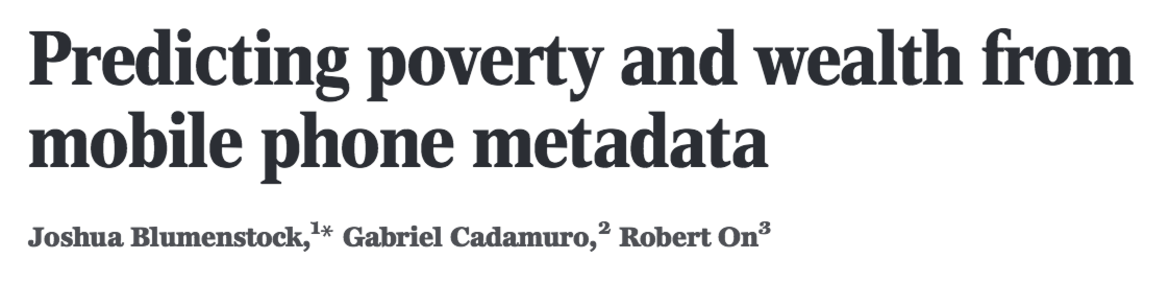
\includegraphics[width=1\textwidth]{figures/blumenstock_predicting_2015_title}
\end{center}

\vf
\tiny{\textcolor{blue}{\url{http://dx.doi.org/10.1126/science.aac4420}}}

\end{frame}
%%%%%%%%%%%%%%%%%%%%%%%%%%%
\begin{frame}{What is computational social science?}

\begin{center}

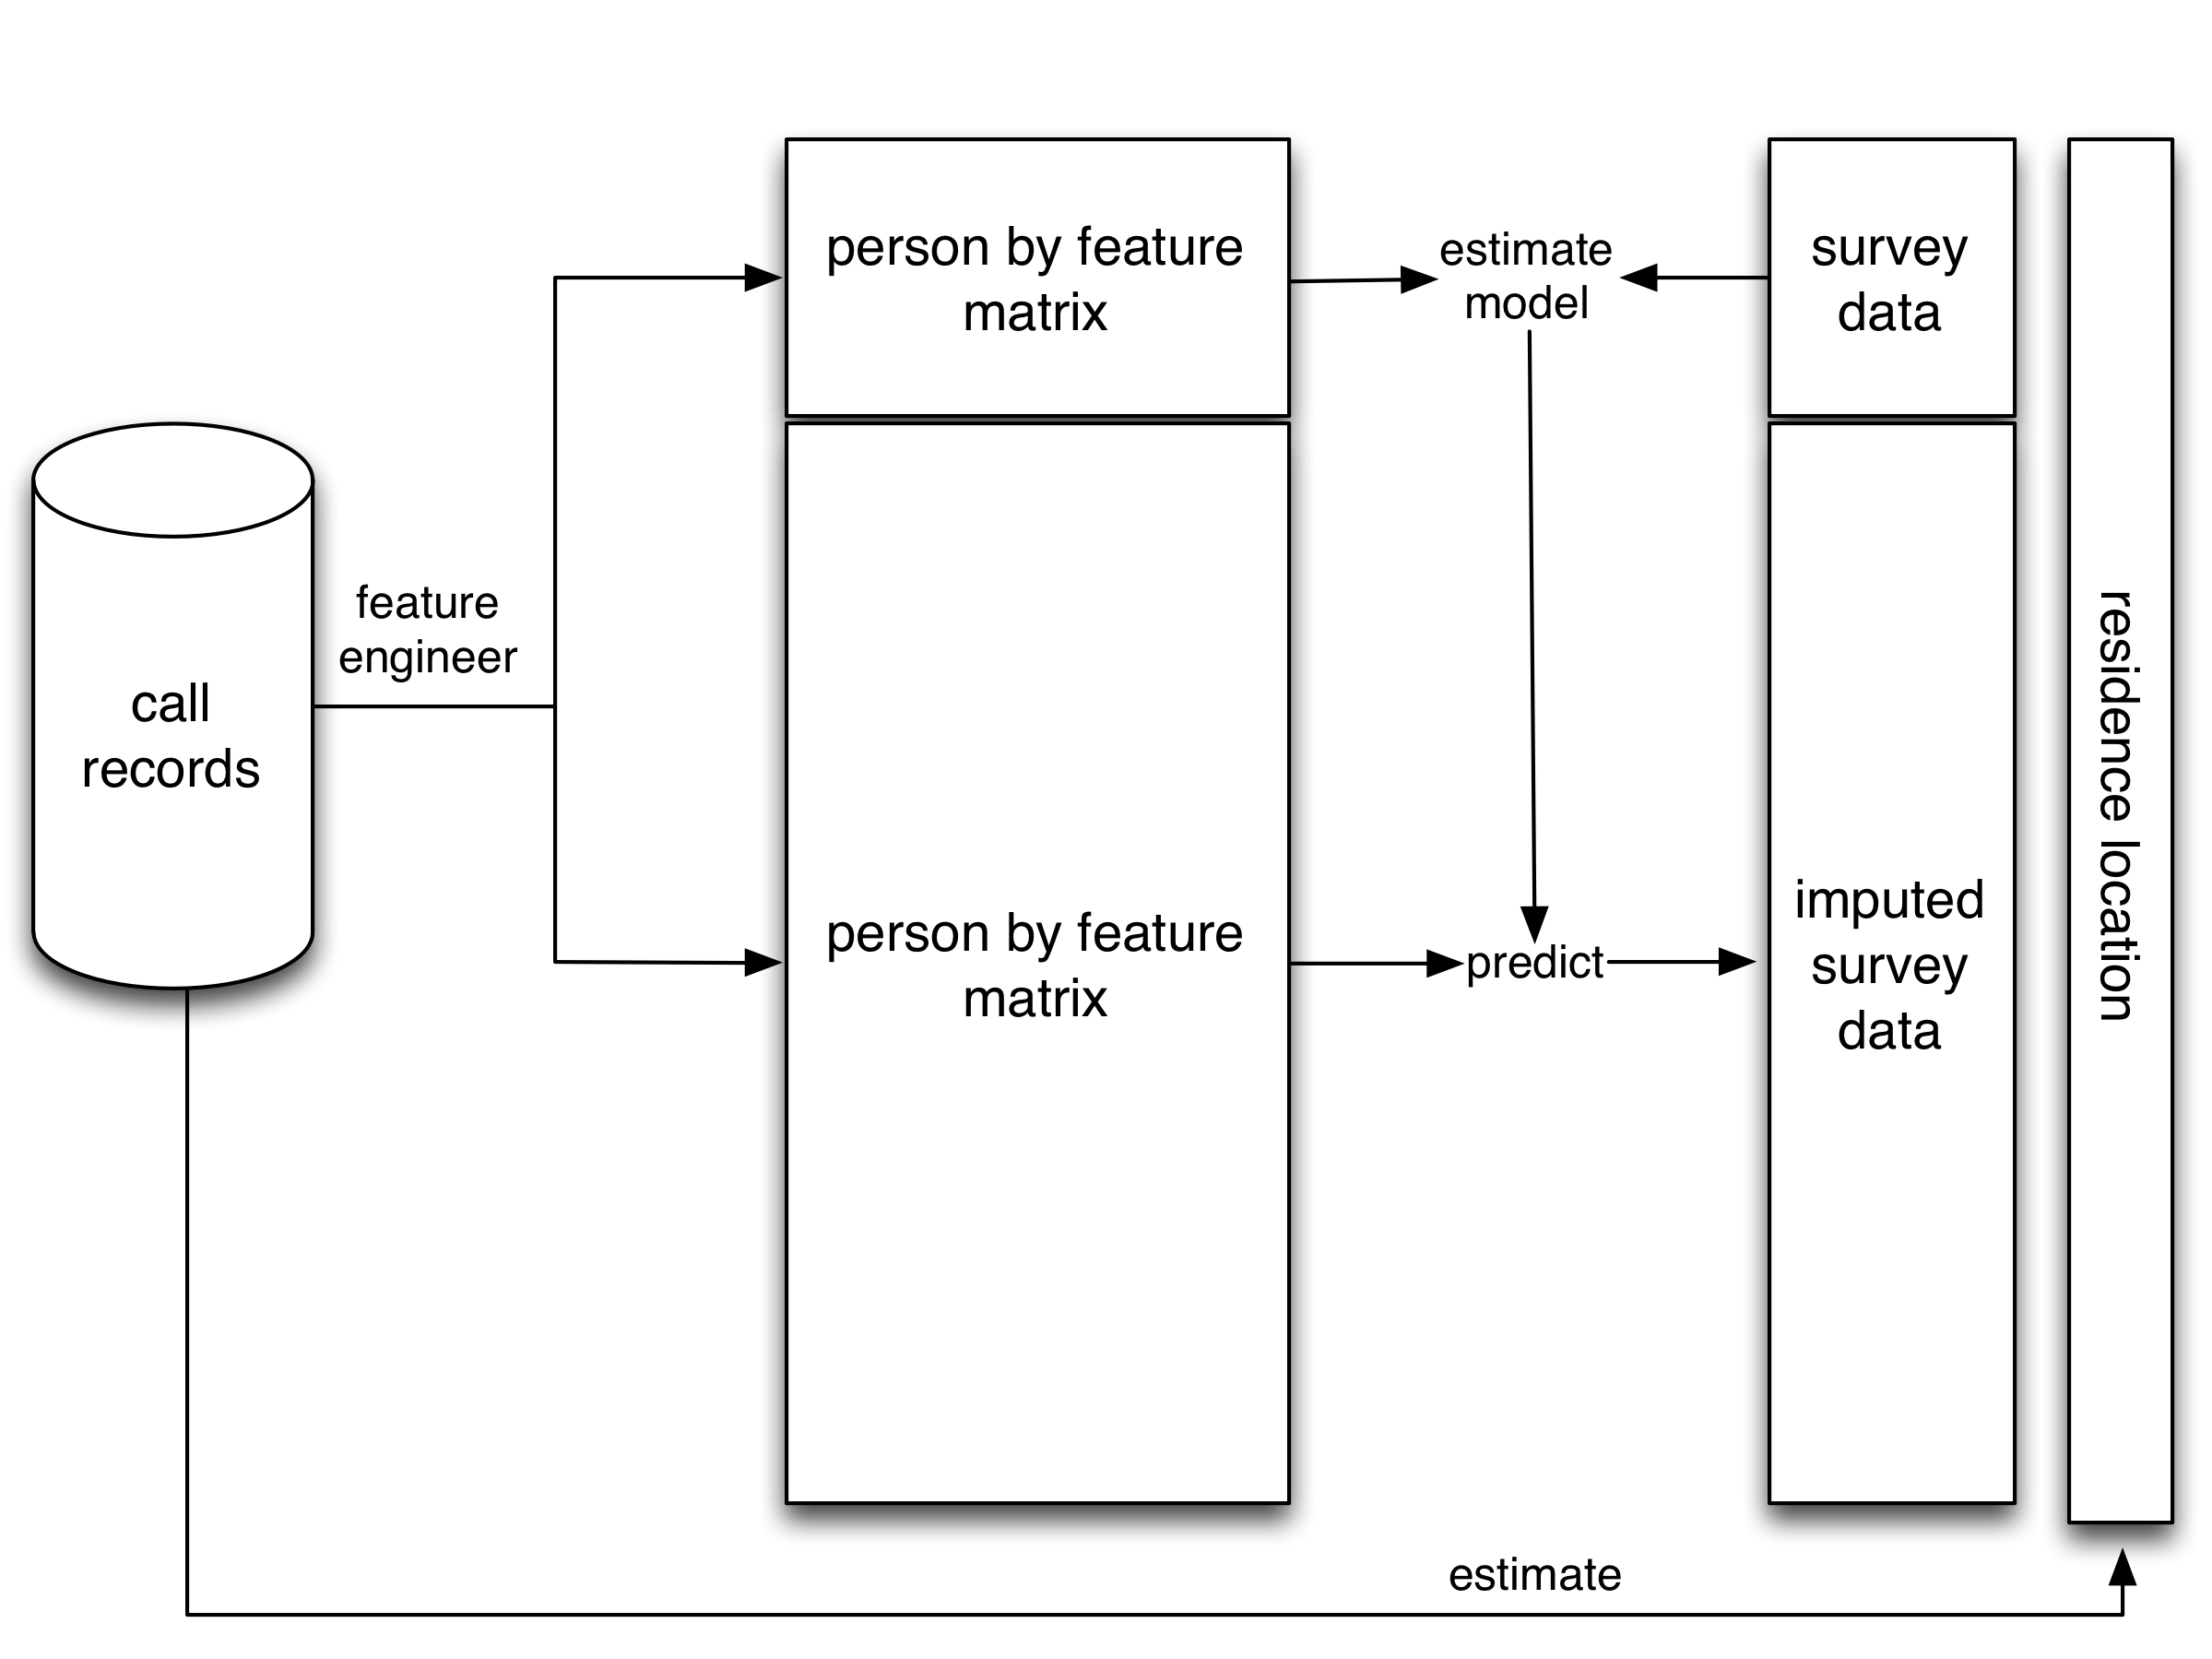
\includegraphics[width=0.9\textwidth]{figures/blumenstock_predicting_2015_schematic_6}
\end{center}

\end{frame}
%%%%%%%%%%%%%%%%%%%%%%%%%
\begin{frame}{What is computational social science?}

\begin{center}
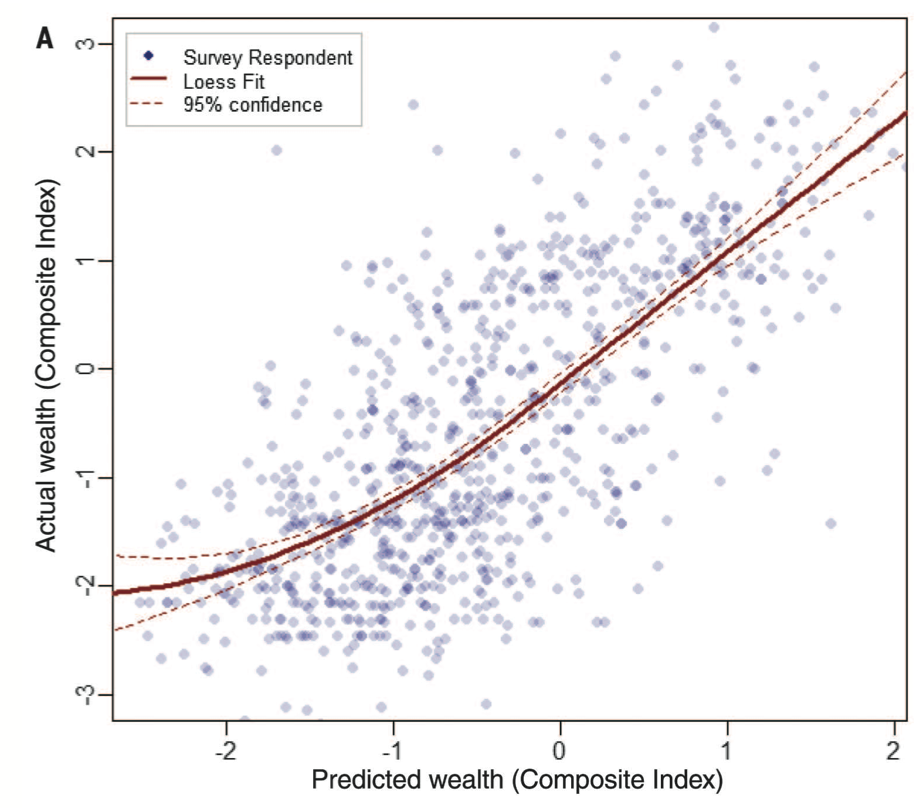
\includegraphics[width=0.7\textwidth]{figures/blumenstock_predicting_2015_fig1a}
\end{center}

\vf
\tiny{\textcolor{blue}{\url{http://dx.doi.org/10.1126/science.aac4420}}}

\end{frame}
%%%%%%%%%%%%%%%%%%%%%%%%%%
\begin{frame}{What is computational social science?}

\begin{center}
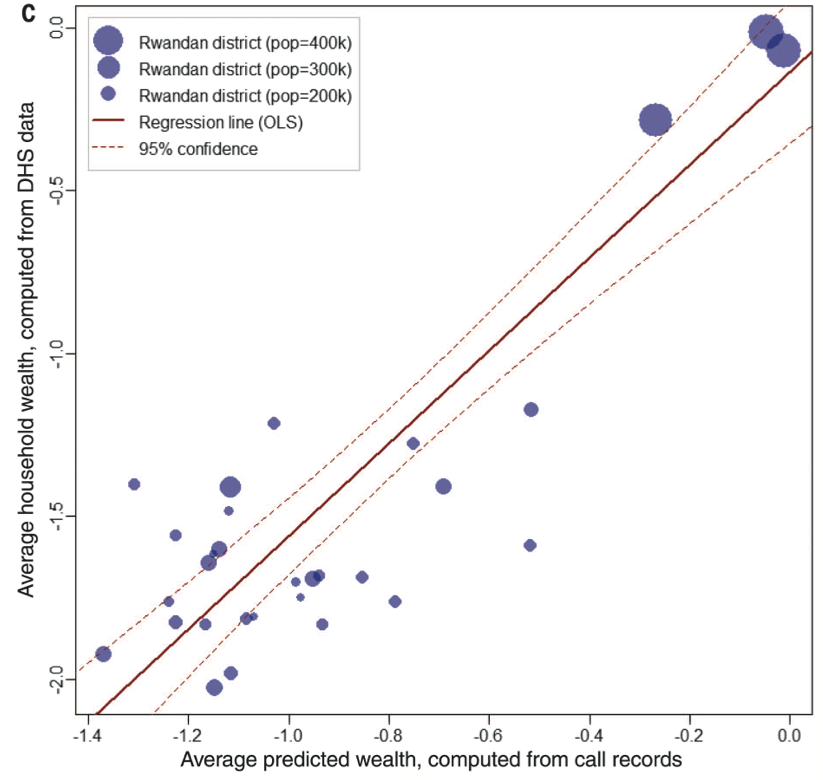
\includegraphics[width=0.60\textwidth]{figures/blumenstock_predicting_2015_fig3c}
\end{center}

%\pause

\begin{center}
	10 times faster, 50 times cheaper
\end{center}

\vf
\tiny{\textcolor{blue}{\url{http://dx.doi.org/10.1126/science.aac4420}}}
\end{frame}
%%%%%%%%%%%%%%%%%%%%%%%%%%
\begin{frame}{What is computational social science?}

\begin{itemize}
\item \emph{computational} and \emph{social science}
%\pause
\item often involves ethical/privacy questions that are now considered complex
%\pause
\item combines readymades and custommades
\end{itemize}

\end{frame}
%%%%%%%%%%%%%%%%%%%%%%%%%%%
\begin{frame}{What is computational social science?}

\begin{center}
\begin{tabular}{ccc}
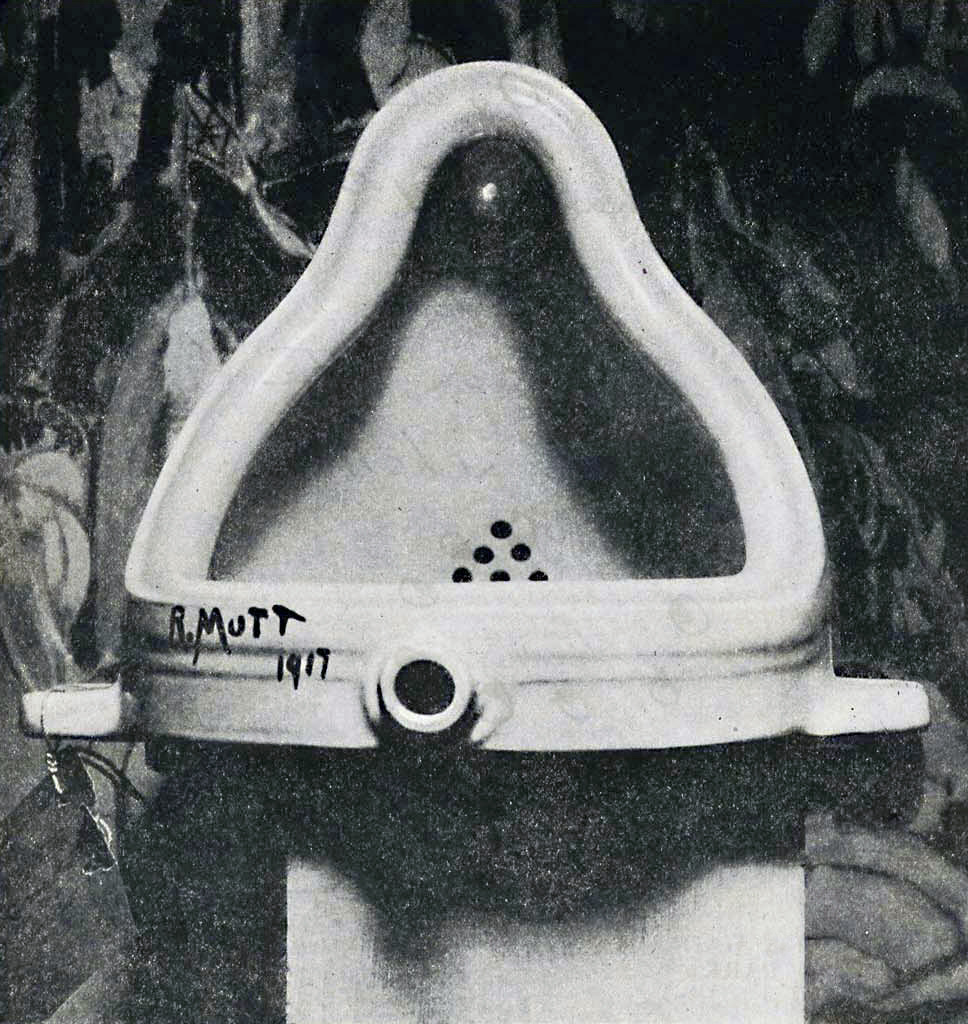
\includegraphics[width=0.30\textwidth]{figures/duchamp_fountain} & \phantom{12345} & {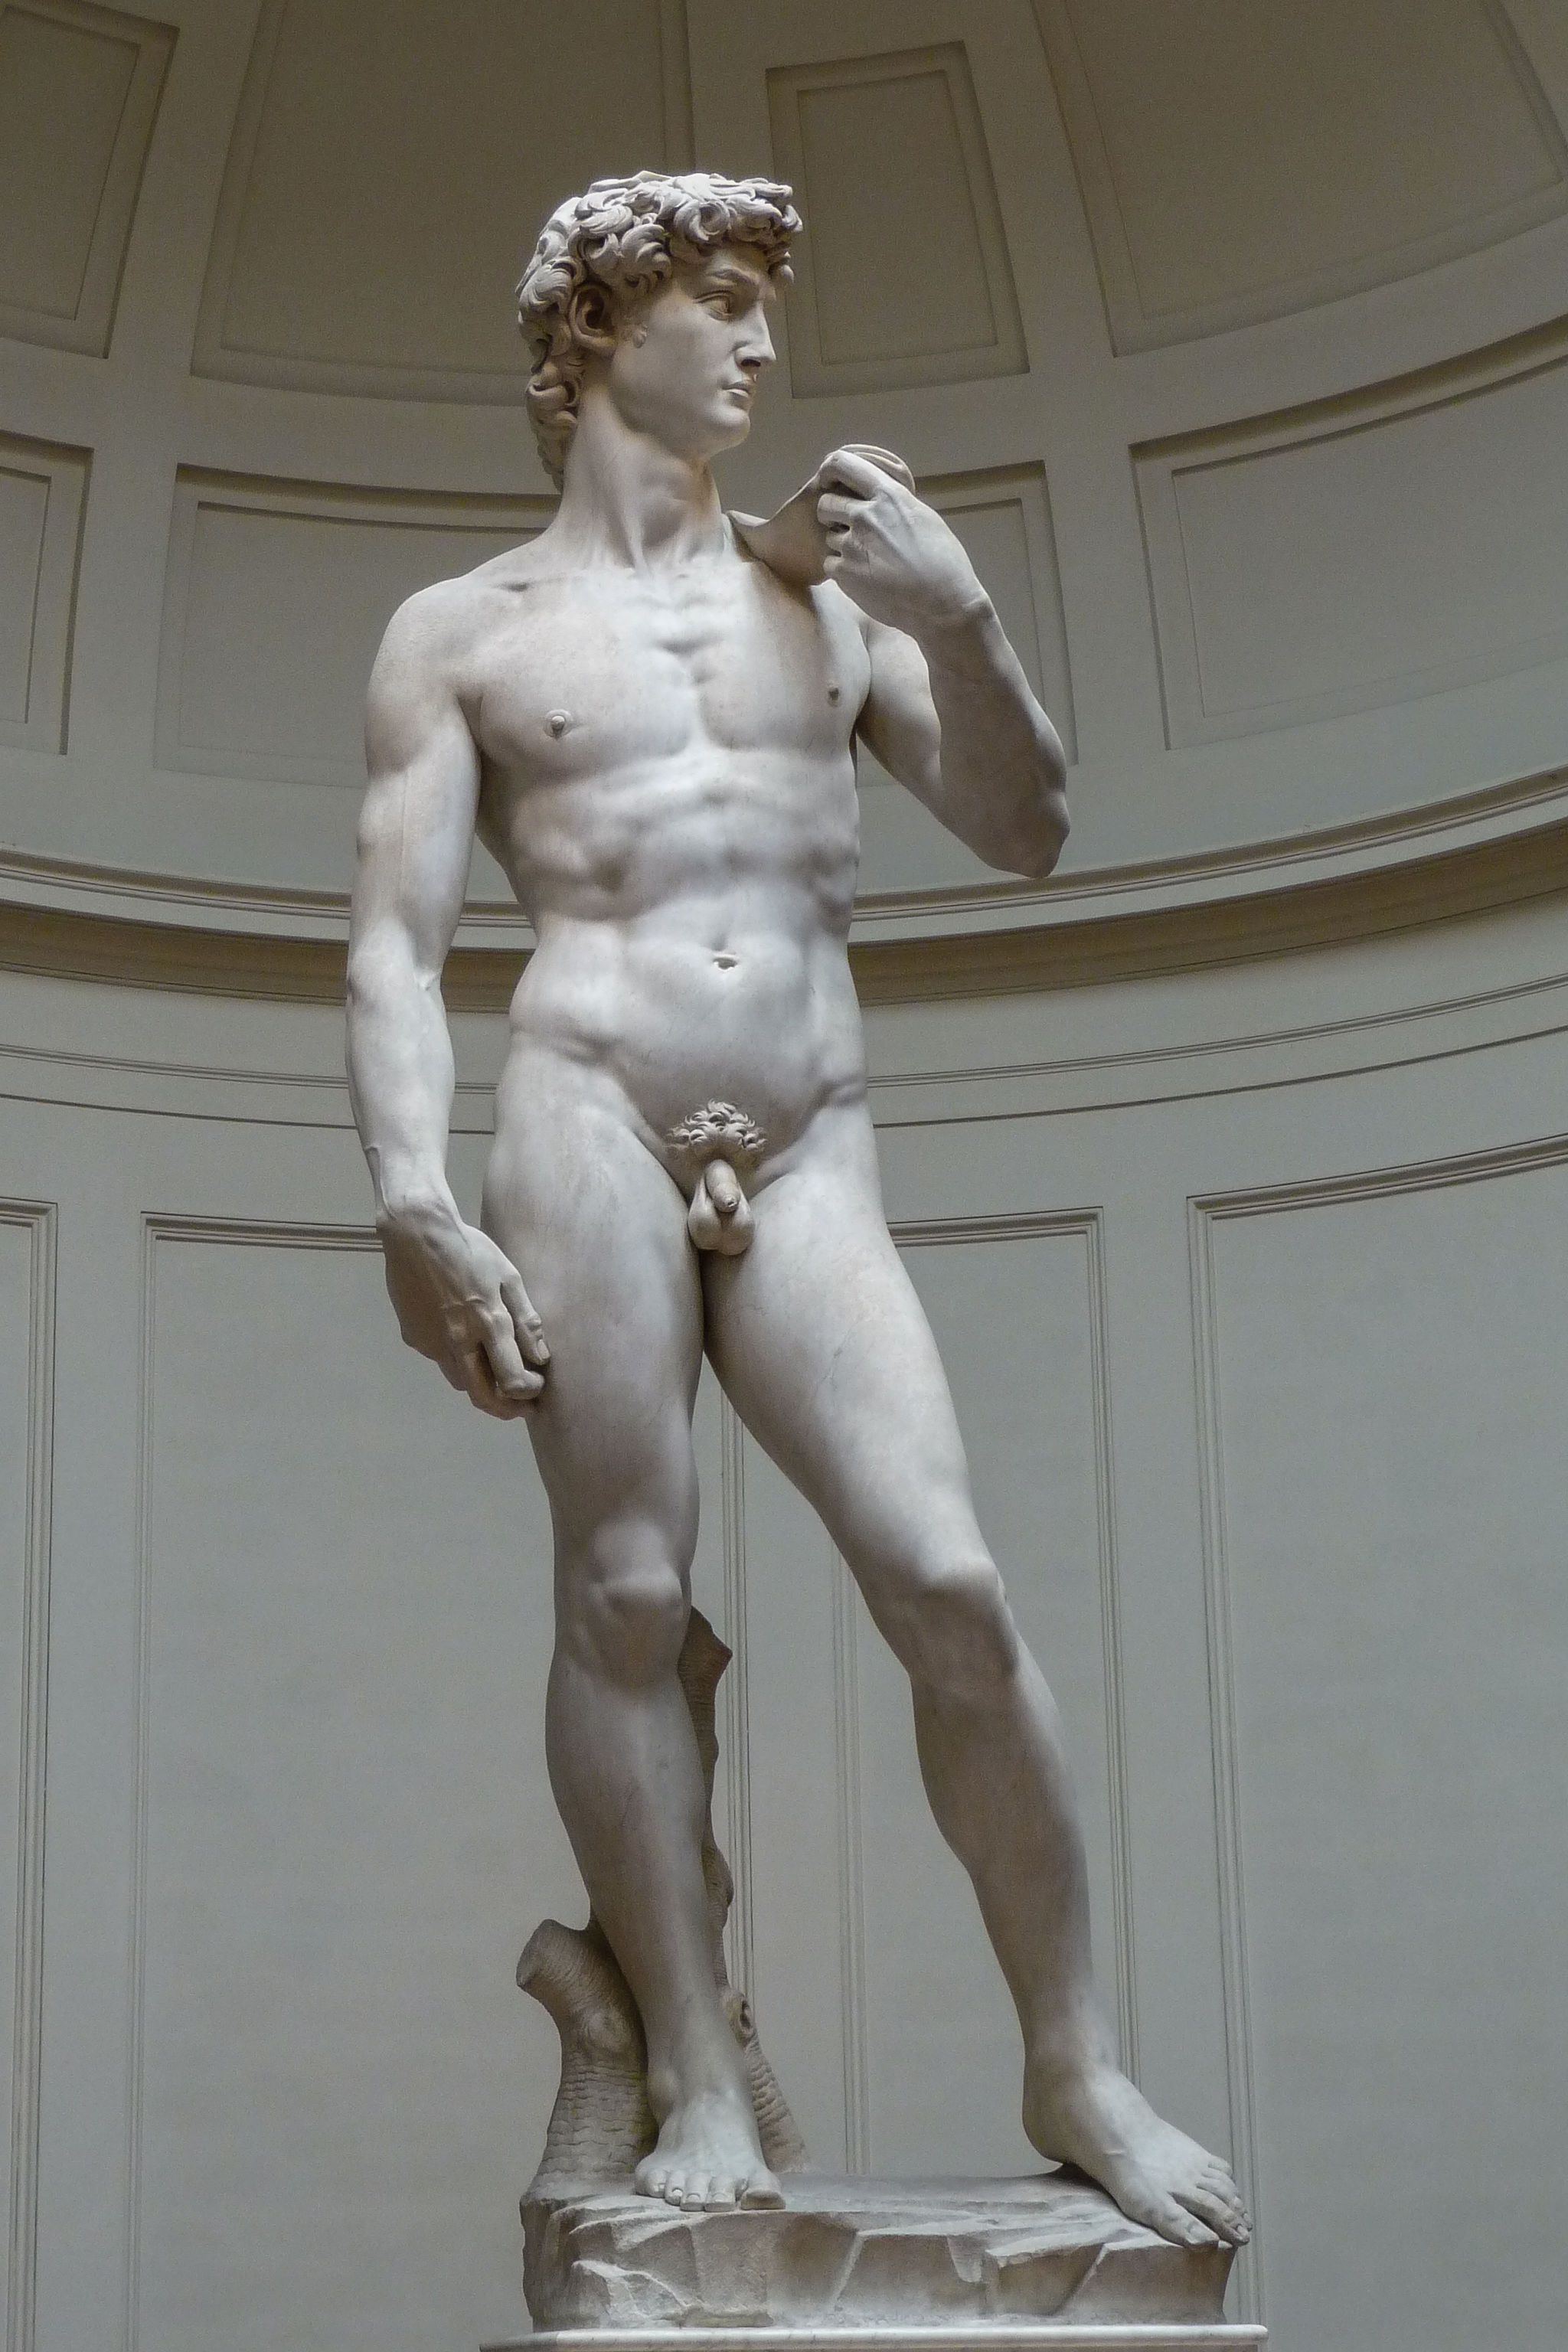
\includegraphics[width=0.30\textwidth]{figures/michelangelo_david}} \\
{\LARGE{readymades}} &  & {\LARGE{custommades}}
\end{tabular}
\end{center}

\vf
{
\tiny{\url{https://commons.wikimedia.org/wiki/File:Duchamp_Fountaine.jpg}}\\
\tiny{\url{https://commons.wikimedia.org/wiki/File:\%27David\%27_by_Michelangelo_JBU0001.JPG}}}

\end{frame}
%%%%%%%%%%%%%%%%%%%%%%%%%%%
\begin{frame}{What is computational social science?}

\begin{itemize}
\item \emph{computational} and \emph{social science}
\item often involves ethical/privacy questions that are now considered complex
\item combines readymades and custommades
%\pause
\item involves five key communities: social science, data science, business people, privacy advocates, policy makers
\end{itemize}

\end{frame}
%%%%%%%%%%%%%%%%%%%%%%%%%%%%
\begin{frame}{What is computational social science?}

\begin{center}
Balance between social science, data science, business people, privacy advocates, and policy makers\\
\end{center}
\vf
\begin{center}
Healthy Ecosystem vs Horrific Monoculture
\end{center}

\end{frame}
%%%%%%%%%%%%%%%%%%%%%%%%%%%
\begin{frame}{What is computational social science?}


\begin{itemize}
\item \emph{computational} and \emph{social science}
\item often involves ethical/privacy questions that are now considered complex
\item combines readymades and custommades
\item involves five key communities: social science, data science, business people, privacy advocates, policy makers
\end{itemize}

\end{frame}
%%%%%%%%%%%%%%%%%%%%%%%%%%%
\begin{frame}{What is computational social science?}

\begin{center}
\LARGE{Isn't computational social science a fad?}
\end{center}

\pause
\begin{center}
	No
\end{center}


\end{frame}
%%%%%%%%%%%%%%%%%%%%%%%%%%%
\begin{frame}{What is computational social science?}

\begin{center}
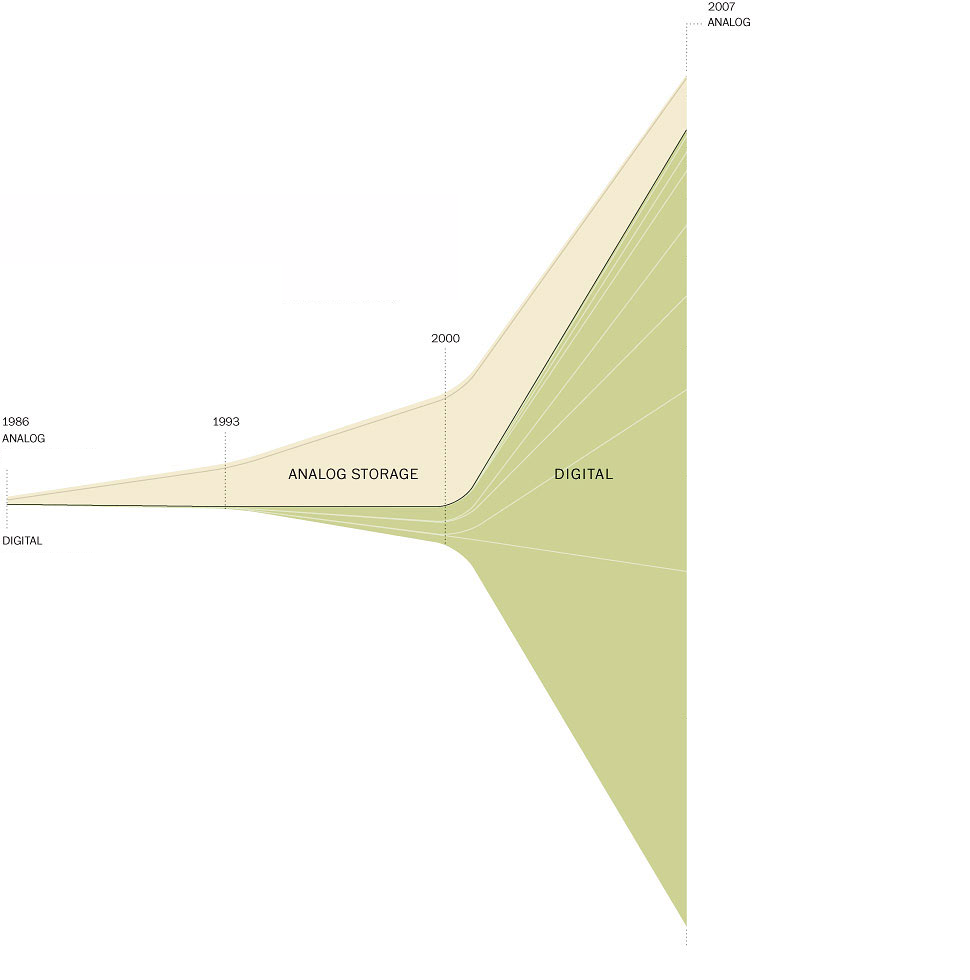
\includegraphics[height=0.8\textheight]{figures/digital_age_clean.png}
\end{center}

\vf
\tiny{\url{http://www.washingtonpost.com/wp-dyn/content/graphic/2011/02/11/GR2011021100614.html}, based on Hilbert and L\`{o}pez (2011)}

\end{frame}
%%%%%%%%%%%%%%%%%%%%%%%%%%%
\begin{frame}{What is computational social science?}

\begin{center}
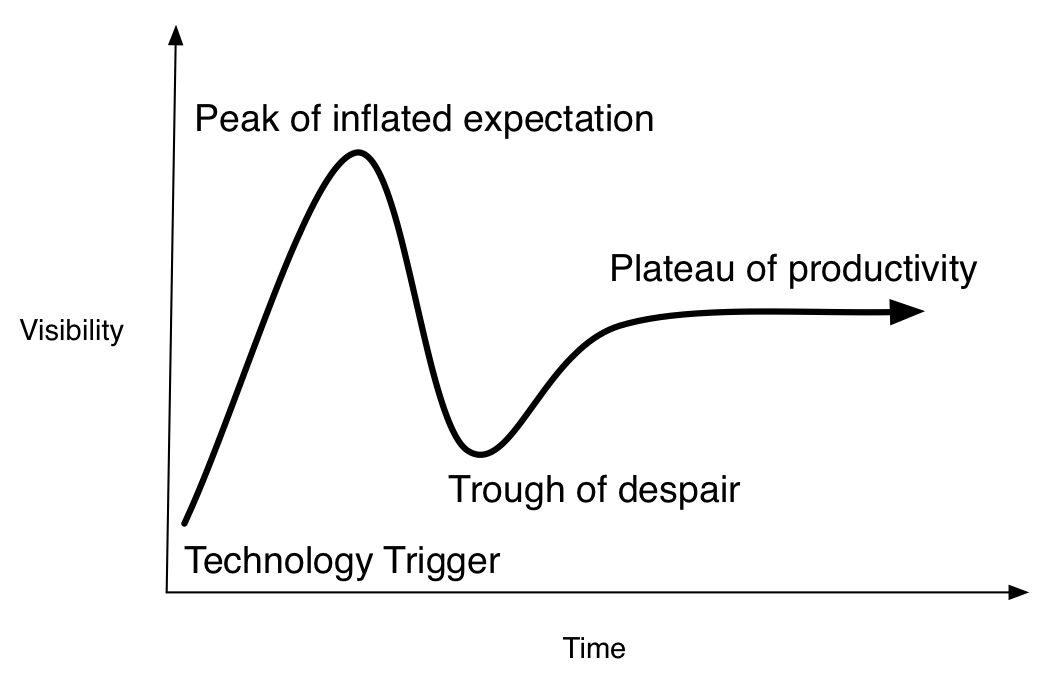
\includegraphics[width=\textwidth]{figures/hype_cycle}
\end{center}

\vf
\tiny{\url{https://commons.wikimedia.org/wiki/File:Gartner_Hype_Cycle.svg}}

\end{frame}
%%%%%%%%%%%%%%%%%%%%%%%%%%%
\begin{frame}{What is computational social science?}

\begin{center}
\LARGE{How do we create computational social science, individually and as a community?}
\end{center}

\end{frame}
%%%%%%%%%%%%%%%%%%%%%%%%%%%%
\begin{frame}{What is computational social science?}

\begin{center}
\LARGE{Social Scientists $\longleftrightarrow$ Data Scientists}
\end{center}

\end{frame}

\section{What is data science?}
%%%%%%%%%%%%%%%%%%%%%%%%%%%

%%%%%%%%%%%%%%%%%%%%%%%%%%%
\begin{frame}{What is data science?}

\begin{center}
\LARGE{Anything that's cool}
\end{center}

\end{frame}
%%%%%%%%%%%%%%%%%%%%%%%%%%%

%%%%%%%%%%%%%%%%%%%%%%%%%%%
\begin{frame}{What is data science?}

\begin{center}
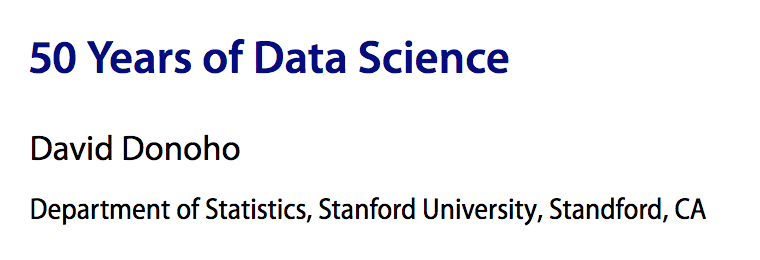
\includegraphics[width=0.8\textwidth]{figures/donoho_50_2017_title.png}\\
\tiny{\textcolor{blue}{\url{https://doi.org/10.1080/10618600.2017.1384734 }}}
\end{center}
%\pause
\vf
\begin{itemize}
\item goes back to Tukey (1962)
%\pause
\item learning from data
%\pause
\item it includes statistics and much more
\end{itemize}

\end{frame}
%%%%%%%%%%%%%%%%%%%%%%%%%%%
\begin{frame}{What is data science?}

\begin{itemize}
\item data science alone is not enough if we want to study social behavior (e.g., Anderson)
%\pause
\item social science alone is not enough if we want to use new data sources
\end{itemize}

\end{frame}
%%%%%%%%%%%%%%%%%%%%%%%%%%%
\begin{frame}{What is data science?}

Hanna Wallach (2015) reports overhearing: ``I don't get it.  Why is that research?''\\
%\pause
\vf
\begin{center}
\begin{tabular}{cc}
Computer science & Social science\\
\midrule
Study anything & Study social things\\
Methods driven & Question driven\\
Large found data & Small designed data\\
Prediction & Explanation\\
\end{tabular}
\end{center}

\vf
\tiny{\url{http://videolectures.net/icml2015_wallach_social_science/}}

\end{frame}
%%%%%%%%%%%%%%%%%%%%%%%%%%%
\begin{frame}{What is data science?}

Another important difference between social science and data science:
\begin{center}
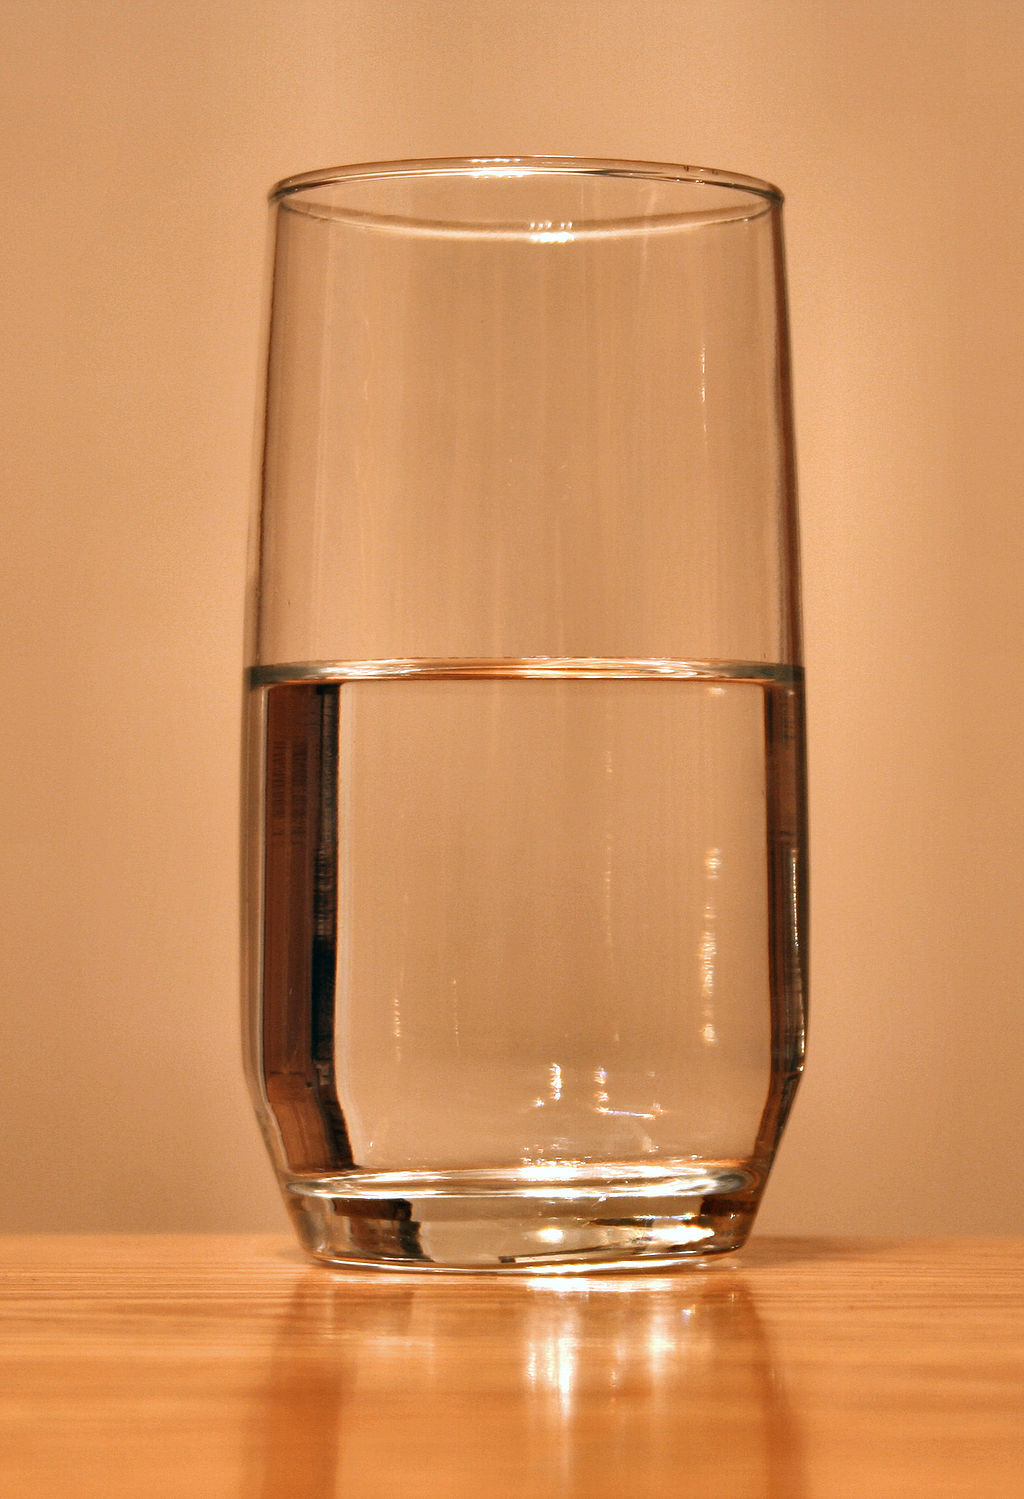
\includegraphics[height=0.7\textheight]{figures/glass-of-water.jpg}
\end{center}

\vf
\vspace{0.5in}
\tiny{\url{https://commons.wikimedia.org/wiki/File:Glass-of-water.jpg}}\\
\end{frame}
%%%%%%%%%%%%%%%%%%%%%%%%%%%
\begin{frame}

\begin{center}
\LARGE{Social Scientists $\longleftrightarrow$ Data Scientists}
\end{center}

\end{frame}
%%%%%%%%%%%%%%%%%%%%%%%%%%%



%%%%%%%%%%%%%%%%%%%%%%%%%%
%%%%%%%%%%%%%%%%%%%%%%%%%%
%%%%%%%%%%%%%%%%%%%%%%%%%%
%%%%%%%%%%%%%%%%%%%%%%%%%%
%%%%%%%%%%%%%%%%%%%%%%%%%%
%%%%%%%%%%%%%%%%%%%%%%%%%%

\end{document}
